% In figure \ref{fig:HD34411_bary_matrix} is plotted the $\Delta V_r^{ij}$ matrix for barycentric-corrected excalibur calibrated data for HD 34411. We are now on the order of m/s instead of km/s.

% \begin{SCfigure}[1][!ht]%
%     \begin{wide}  
%         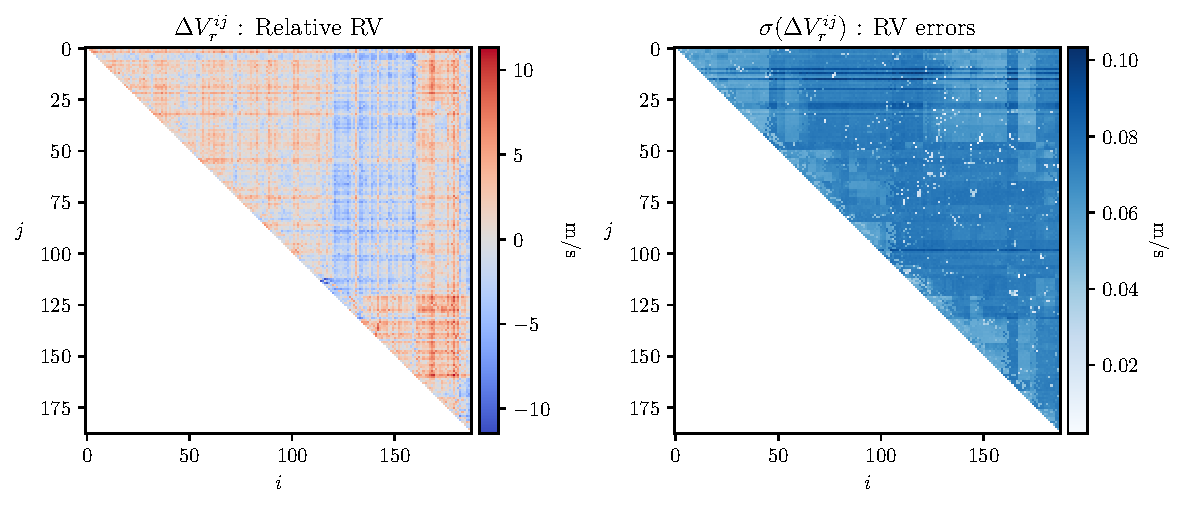
\includegraphics[width=\textwidth]{figures/HD34411_bary_matrix.pdf}
%         \caption{RV shifts matrix computed for HD34411 using excalibur calibrated, barycentric-corrected data (column \texttt{bary\char`_excalibur}). Each cell shows the median relative radial velocity across all features found between observations $i$ and $j$.}
%         \label{fig:HD34411_bary_matrix}
%     \end{wide}
% \end{SCfigure}

Figure \ref{fig:HD34411_rvs} shows my extracted relative radial velocity results for HD 34411 compared to those of Lily Zhao et al (also available upon request \cite{yale_data}). As the Earth's movement has been removed, we are now on the scale of m/s instead of km/s. The method used by Lily Zhao et al is a "chunk-by-chunk" method, where each spectrum is split into ~2Å chunks for each of which an RV is found by shifting a template spectrum to match the observed spectrum. That is to say, a different method from mine. Our results however coincide within the same order of magnitude and with a similar rms of 1.67 m/s and 1.78 m/s, mine and hers respectively. The residuals however do jump arund quite a bit, and, of course, my mean error of 0.8 cm/s is not correct.

\begin{SCfigure}[1][!ht]%
    \begin{wide}  
        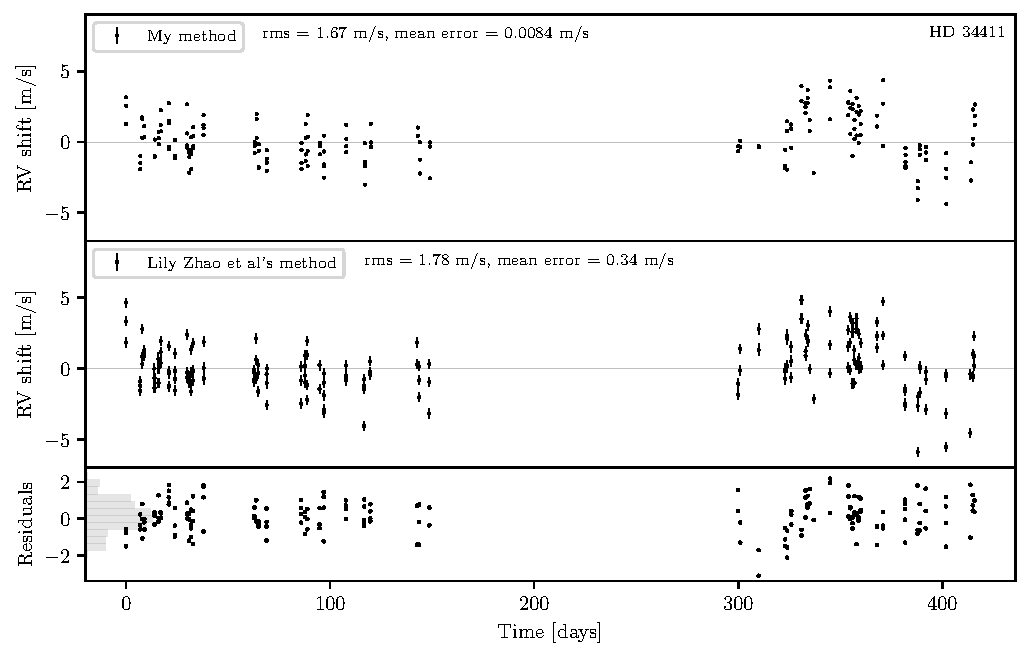
\includegraphics[width=\textwidth]{figures/HD34411_barycentric_rv_vs_lily.pdf}
        \caption{Top: my final extracted RV shifts for HD 34411 using excalibur calibrated, barycentric-corrected data (data column \texttt{bary\char`_excalibur}). Center: Lily Zhao et al's results using a chunk-by-chunk (CBC) analysis technique \cite{yale_data}. Bottom: residuals from subtracting Lily's results from mine. 188 observations made between 2019-10-8 and 2020-11-27.}
        \label{fig:HD34411_rvs}
    \end{wide}
\end{SCfigure}

I've analysed data from three more stars and again compared the results with those of Lily et al. As with HD 34411, my rms values come within a few m/s, the residuals are not small, and my errors are too small. See figures \ref{fig:HD101501_rvs}, \ref{fig:HD10700_rvs} and \ref{fig:HD26965_rvs} in appendix \ref{appendix:results} for plots. 
